\subsection{Unsupervised Clustering \label{sec:unsupervised_clustering}}

\subsubsection{Method}

The idea is to unsupervisely evaluate the agglomerative clustering at each number of clusters (at each merge step).
When discarding clustering with $N$ and clusters $1$, this produce $N - 2$ possible clusterings, each of those are evaluated using the mean Silhouette score.
See Definition~\ref{def:silhouette}.

\begin{definition}[Mean Silhouette score~\cite{sklearn}~\cite{wiki_silhouette}]
  \label{def:silhouette}
  The mean Silhouette score is an unsupervised clustering metric which evaluate a clustering result by measuring the cohesion and separation of the clusters.
  \begin{equation}
    s = \frac{1}{|C|} \sum_{i = 0}^{|C|} \frac{b(i) - a(i)}{max(a(i), b(i))}
  \end{equation}
  \begin{equation}
    \begin{split}
      a(i)&: \text{mean intra-cluster distance} \\
      a(i)& = \frac{1}{|C_i| - 1} \sum_{j \in C_i, i\neq j} d(i, j) \\
      b(i)&: \text{mean nearest-cluster distance} \\
      b(i)& = \min_{k\neq i} \frac{1}{|C_k|} \sum_{j \in C_k} d(i, j) \\
    \end{split}
  \end{equation}
  With $C$ the set of clusters, $C_i$ the i-th cluster, $d(i, j)$ the distance between the document i and j.
  $d(i, j)$ are pre-computed and used for the rank list.
  The value is ranged between -1 and 1, a large value indicate a good cohesion and good separation of the clusters (low intra-cluster distance, high nearest-cluster distance).
\end{definition}

The idea is to apply the hierarchical clustering at each possible number of clusters (from $N - 1$ to $2$), and compute the mean Silhouette score.
The best clustering is the one which have the largest mean Silhouette score.
An alternative to this method is the Iterative Positive Silhouette (IPS) and was proposed in Layton, Watters, Dazeley (2011)~\cite{automated_unsupervised}.

\subsubsection{Evaluation}

For this experiment, the goal is to test the unsupervised hierarchical clustering cut method based on the maximization of the mean silhouette score on the literature corpora.
The right number of cluster is not known.
When applying the procedure, the number of clusters start at 2 and end at the number of documents minus 1.
The best clustering according to this method is the one that yield the greatest mean silhouette score, ref. Section~\ref{sec:unsupervised_clustering}.

The rank list used for this experiment is the one generated using Z-Score fusion with retained text representation (9 for St-Jean and 7 for Brunet and Oxquarry), see Section~\ref{sec:annex_retained_text_representation} in annex.

The detailed $B^3_{F_1}$ and score on the unsupervised clustering is presented in Table~\ref{tab:unsupervised_clustering_alpha}.
An example of the best case and worse case are presented Figures~\ref{fig:unsupervised_clustering}.
The silhouette score is indicated as each step and compared to clustering evaluation metrics.

Since the rank lists used for the clustering are not perfect (every true links at the top), there can't be a number of cluster with a BCubed $F_1$ score of 1.0.
The average r-ratio difference is positive value ranging between $\left[0.16, 0.20\right]$ depending on the linkage criterion which indicate that estimated number of cluster is on every dataset overestimated, which means that the mean neareast-cluster distance is greater than the mean intra-cluster distance even when dealing with the right number of clusters.
This can be due to the fact that the rank list used for the clustering is not perfect (AP $\neq 1$).

To mitigate this problem, an easy solution would be to use the labels produced by the clustering of a non-maximal value of the silhouette score on the left side of the maximal silhouette score.
In this study, we introduce a parameter called $\alpha$.
$\alpha$ represents a percentage of value to subtract to the maximal mean silhouette score to obtain the new target (instead of the maximal value).
The clustering with the silhouette score the closest to the target is retained.
The sign of the alpha indicate on the side of the maximal silhouette score the target should be.
With $\alpha = 0$, this corresponds to the maximal mean silhouette score.
With a negative $\alpha$ the left side is targeted and with a positive $\alpha$, the right side.
By using for example $\alpha = -0.2$, we aim to correct this overshoot.
This value was choosen using a grid search to optimize the $B^3_{F_1}$.
Table~\ref{tab:unsupervised_clustering_alpha} show the results with $\alpha = -0.2$.
With this correction technique, in average the $r_{diff}$ is close to 0 and the average $B^3_{F_1}$ is increased in average by 15\% across all the corpora.
The average linkage criterion give the best results for this clustering method, the $B^3_{F_1}$ is in average 3\% better with this technique.

\begin{table}
  \centering
  \caption{Unsupervised clustering evaluation on every linkage criterion and corpus}
  \label{tab:unsupervised_clustering}

  \subcaption{Silhouette maximization ($\alpha = 0$)}
  \label{tab:unsupervised_clustering_0}

  \resizebox{\linewidth}{!}{
  \begin{tabular}{l c c c}
    \toprule
           & \multicolumn{3}{c}{Linkage criterion} \\
    Corpus    & Single     & Average   & Complete \\
    \midrule
    Oxquarry  & 0.80/0.10 & 0.80/0.10 & 0.80/0.10 \\
    Brunet    & 0.67/0.32 & 0.72/0.20 & 0.70/0.25 \\
    St-Jean A & 0.57/0.30 & 0.57/0.29 & 0.60/0.25 \\
    St-Jean B & 0.89/0.08 & 0.91/0.05 & 0.91/0.05 \\
    \midrule
    Absolute mean & 0.73/0.20 & 0.75/0.16 & 0.75/0.16 \\
    \bottomrule
  \end{tabular}
  }

  \vspace{0.5cm}

  \subcaption{$\alpha = -0.2$}
  \label{tab:unsupervised_clustering_alpha}
  \resizebox{\linewidth}{!}{
  \begin{tabular}{l c c c}
    \toprule
           & \multicolumn{3}{c}{Linkage criterion} \\
    Corpus    & Single     & Average   & Complete \\
    \midrule
    Oxquarry  & 0.85/0.02 & 0.96/0.02 & 0.87/0.04 \\
    Brunet    & 0.82/0.05 & 0.85/0.09 & 0.82/0.11 \\
    St-Jean A & 0.77/0.13 & 0.79/0.12 & 0.74/0.12 \\
    St-Jean B & 0.92/-0.01 & 0.89/-0.03 & 0.91/-0.03 \\
    \midrule
    Absolute mean & 0.84/0.05 & 0.87/0.07 & 0.84/0.08 \\
    \bottomrule
  \end{tabular}
  }
\end{table}

\begin{figure}
  \caption{Unsupervised clustering example the worse (St-Jean A) and best (St-Jean B) clustering with the average linkage criterion}
  \label{fig:unsupervised_clustering}

  \subcaption{St-Jean A}
  \label{fig:unsupervised_clustering_st_jean_A_average}
  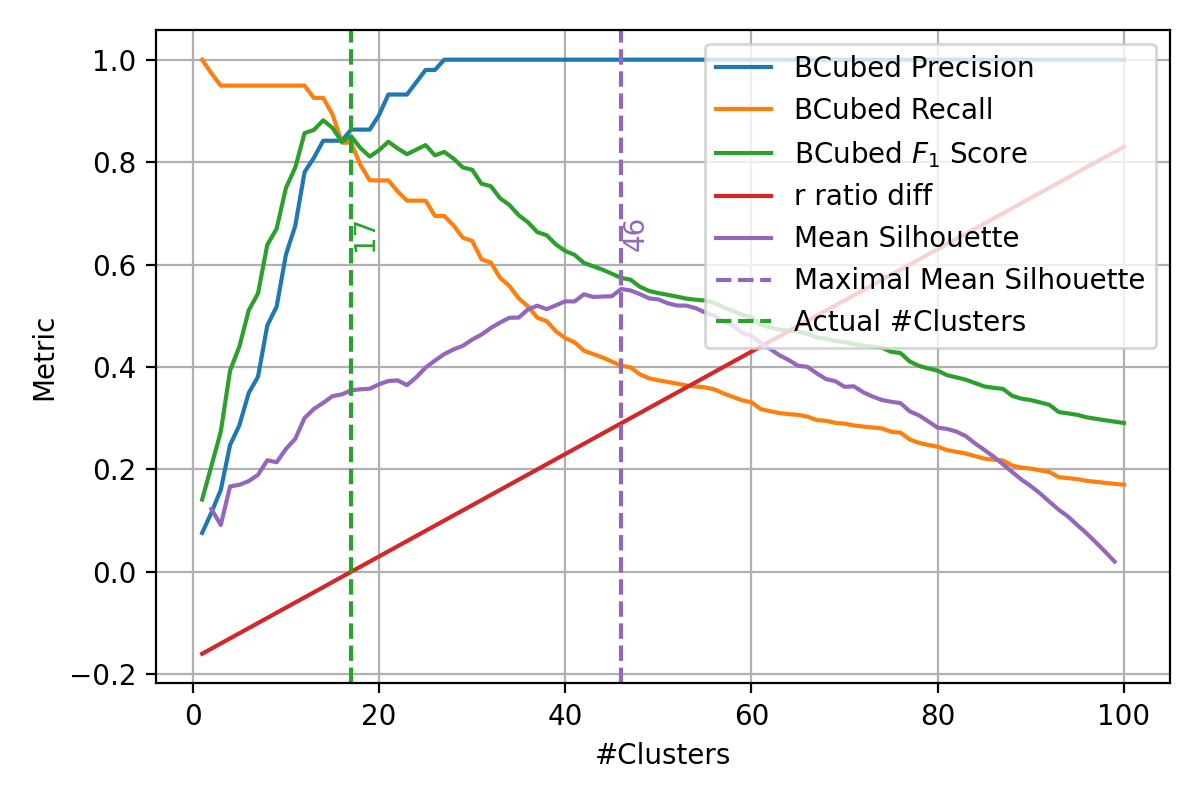
\includegraphics[width=\linewidth]{img/unsupervised_clustering_st_jean_A_average.png}

  \vspace{0.5cm}

  \subcaption{St-Jean B}
  \label{fig:unsupervised_clustering_st_jean_B_average}
  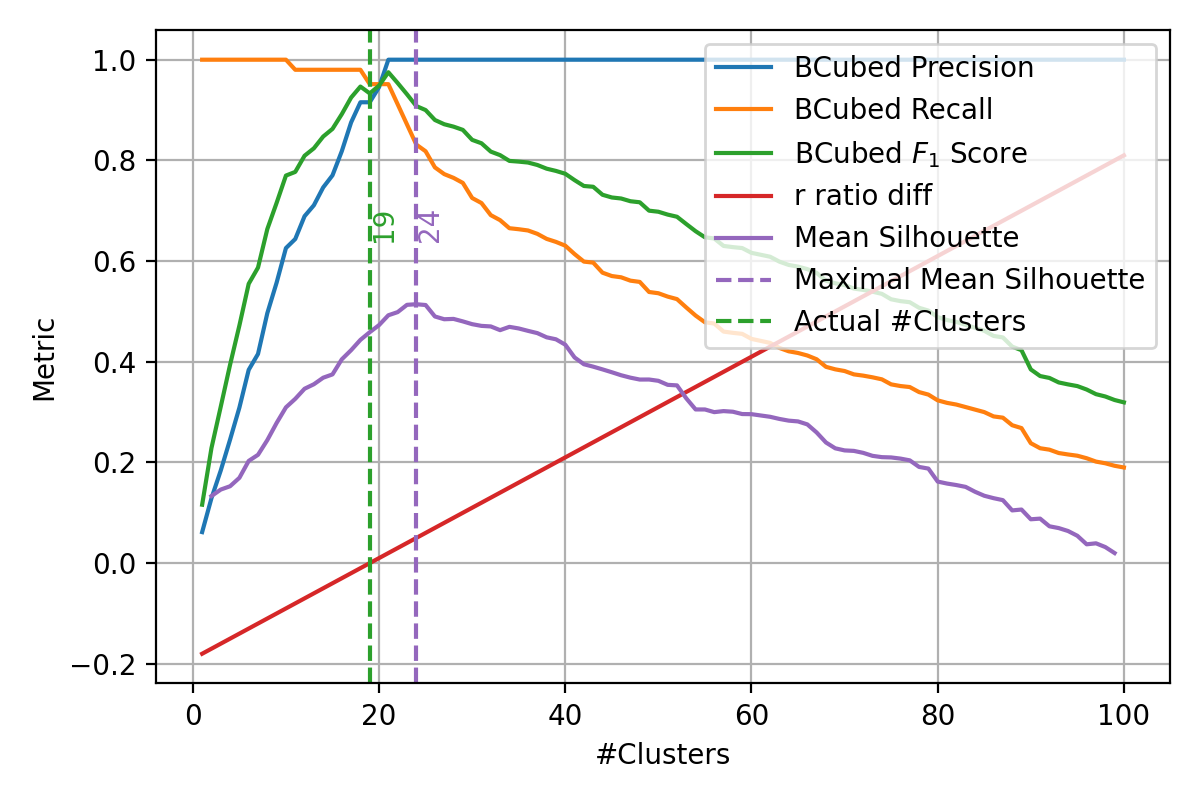
\includegraphics[width=\linewidth]{img/unsupervised_clustering_st_jean_B_average.png}
\end{figure}
